سوال ۲

\subsection*{۱.۲}

برای ماشین متناهی غیرقطعی داده شده، ماشین متناهی قطعی‌ای طراحی کردیم که پذیره‌ی همان زبان است صرفا. (رشته‌های عضو زبان را می‌پذیرد و رشته‌های غیرعضو زبان را نمی‌پذیرد.)

در ابتدا استیت‌ها و تابع انتقال DFA مذکور را می‌نویسیم.

\begin{table}[H]
	\centering
	\begin{tabular}{c|c|c}
		q & \(\delta(q, a)\) & \(\delta(q, b)\)\\
		\hline
		$1256 & 12356 & 576$\\
		$12356 & 12356 & 5674$\\
		$576 & 6 & 576$ \\
		$5674 & 6 & 5672$ \\
		$5762 & 63 & 576$ \\
		$6 & \O & 7$ \\ 
		$7 & 6 & \O$ \\
		$63 & \O & 74$ \\
		$74 & 6 & 2$ \\
		$2 & 3 & \O$ \\
		$3 & \O & 4$ \\
		$4 & \O & 2$ \\
		\(\emptyset\) & \(\emptyset\) & \(\emptyset\)
	\end{tabular}
\end{table}

حالا از Alphabet استفاده می‌کنیم برای ساده‌سازی.

\begin{table}[H]
	\centering
	\begin{tabular}{c|c|c}
		q & \(\delta(q, a)\) & \(\delta(q, b)\)\\
		\hline
		A & B & C  \\    
		B & B & D \\ 
		C & E & C \\ 
		D & E & F \\
		F & G & C \\ 
		E & \O & H \\ 
		H & E & \O \\ 
		G & \O & I \\
		I & E & J \\
		J & K & \O \\
		K & \O & L \\
		L & \O & J \\ 
		\O & \O & \O
	\end{tabular}
\end{table}

حالا DFA این NFA را می‌کشیم.

\\
\\
\begin{center}
	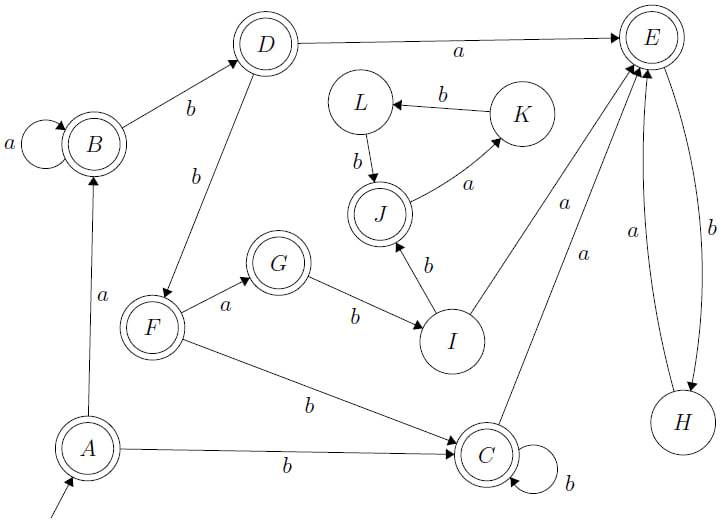
\includegraphics{DFA5}
\end{center}

\subsection*{۲.۲}

برای این کاهش جدول مثلثی شکلی تشکیل می‌دهیم و سطر و ستون‌های شامل استیت‌های فاینال را دایره می‌کشیم. در نهایت هر دو استیت را بررسی می‌کنیم. 

\\
\\
\begin{center}
	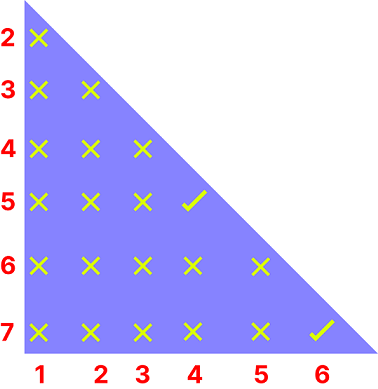
\includegraphics{list}
\end{center}

حالا unreachable نداریم پس کافی‌ست حالات مشابه را فقط در نظر بگیریم. در این‌جا حالات ۴ و ۵ و همچنین ۶ و ۷ مشابه هستند پس DFA آن را می‌کشیم.

\begin{center}
	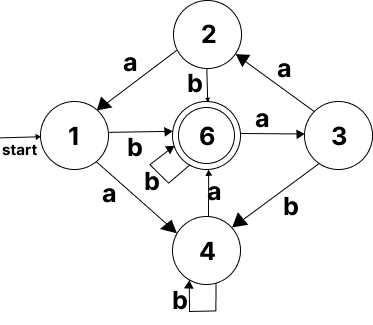
\includegraphics{DFA6}
\end{center}

